\begin{frame}
  \frametitle{Algorithm, Experiments \& Conclusion}

  \uncover<3->{%
    \ribbon[\paperwidth][black][VectorPink]{ \centering \textbf{Our KFAC-based optimizer outperforms popular methods, scales to large neural networks, and performs similarly to Hessian-free {\scriptsize \citep[][ICML]{martens2010deep}}}.}
  }

  \begin{columns}
    \begin{column}[b]{0.34\linewidth}
      \vspace{-1.5ex}
      \begin{align*}
        L(\vtheta) = L_{\Omega}(\vtheta) + L_{\partial\Omega}(\vtheta)
      \end{align*}
      \vspace{-3ex}

      \begin{itemize}
      \item \emph{Goal:} Approximate Gauss-Newton matrix
        \vspace{-1ex}
        \begin{align*}
          \mG(\vtheta) = \mG_{\Omega}(\vtheta) + \mG_{\partial\Omega}(\vtheta)
        \end{align*}

        \vspace{-1ex}

        \uncover<2->{
        \item \emph{KFAC}
          \vspace{-1.5ex}
          \begin{align*}
            G_{\Omega}(\mW)
            &\approx \mA_{\Omega} \otimes \mB_{\Omega}
              \shortintertext{(generalized to diff.\,ops)}
              G_{\partial\Omega}(\mW)
            &\approx \mA_{\partial\Omega} \otimes \mB_{\partial\Omega}
              \shortintertext{{\scriptsize\citep[][ICML]{martens2015optimizing}}}
          \end{align*}
        }
      \end{itemize}
    \end{column}
    \begin{column}[b]{0.7\linewidth}
      \centering
      \uncover<3->{%
        \begin{minipage}{0.49\linewidth}
          \centering
          4+1d heat, $D \approx 10^5$

          % [trim={left bottom right top},clip]
          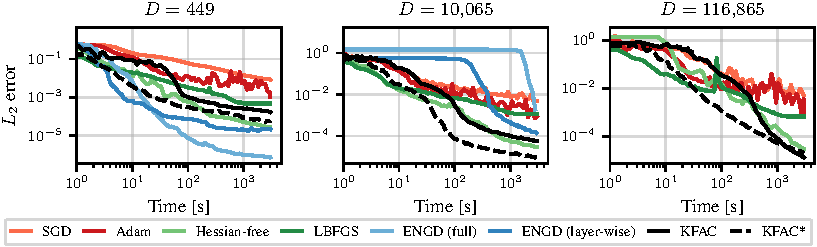
\includegraphics[trim={9.5cm 0.9cm 0 0.3cm},clip, width=0.70\linewidth]{../kfac_pinns_exp/exp30_heat4d_groupplot/l2_error_over_time.pdf}
        \end{minipage}
      }
      \hfill
      \uncover<3->{%
        \begin{minipage}{0.49\linewidth}
          \centering
          100d Poisson, $D\approx 10^6$

          % [trim={left bottom right top},clip]
          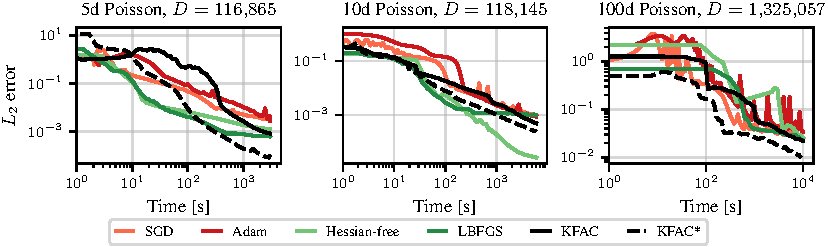
\includegraphics[trim={9.5cm 0.9cm 0 0.3cm},clip, width=0.70\linewidth]{../kfac_pinns_exp/exp33_poisson_bayes_groupplot/l2_error_over_time.pdf}
        \end{minipage}
      }

      \vspace{-1ex}

      \uncover<3->{
        \begin{center}
          9+1d log Fokker-Planck, $D \approx 10^5$

          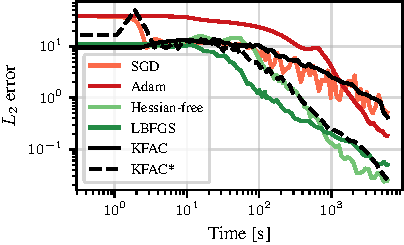
\includegraphics[width=0.45\linewidth]{../kfac_pinns_exp/exp43_log_fokker_planck9d_isotropic_gaussian_random/l2_error_over_time.pdf}
        \end{center}
      }
      \vspace*{3.5ex}
    \end{column}
  \end{columns}
\end{frame}
%%% Local Variables:
%%% mode: LaTeX
%%% TeX-master: "../pitch"
%%% End:
